% Day 4 notes, SC Quantathon v3 Bootcamp. Build: latexmk -pdf notes.tex
\documentclass[11pt]{article}

\usepackage[margin=1in]{geometry}
\usepackage{lmodern}
\usepackage[T1]{fontenc}
\usepackage{microtype}
\usepackage{amsmath,amssymb}
\setlength{\arraycolsep}{3pt}
\usepackage{braket}
\usepackage{graphicx}
\usepackage{booktabs}
\usepackage{caption}
\usepackage{listings}
\usepackage{xcolor}
\usepackage[hidelinks]{hyperref}

\captionsetup{font=small,labelfont=bf}
\graphicspath{{figures/}}

\lstset{
  language=Python,
  basicstyle=\ttfamily\small,
  keywordstyle=\color{blue!60!black},
  commentstyle=\color{gray},
  stringstyle=\color{green!40!black},
  showstringspaces=false,
  frame=single,
  framerule=0.3pt,
  rulecolor=\color{gray!50},
  xleftmargin=1em,
  aboveskip=0.6em,
  belowskip=0.6em,
}

\newcommand{\code}[1]{\texttt{#1}}

\title{Day 4: Gates, Measurement, and Entanglement}
\author{SC Quantathon v3 Bootcamp \\ Clemson Quantum Club}
\date{}

\begin{document}
\maketitle

\noindent
Day~2 established that a qubit is a point on the Bloch sphere and that a gate is a unitary matrix. These notes complete the single-qubit toolkit, rotations by any angle, gate composition, measurement in any basis, and expectation values, and then add the second qubit, which brings the tensor product, the CNOT gate, and the one thing two qubits can do that no pair of classical bits can, which is to be entangled. They follow the Day~4 notebook section by section.

\section{The Pauli gates as half-turns}

The three Pauli matrices
\begin{equation}
X = \begin{pmatrix}0&1\\1&0\end{pmatrix},\qquad
Y = \begin{pmatrix}0&-i\\i&0\end{pmatrix},\qquad
Z = \begin{pmatrix}1&0\\0&-1\end{pmatrix}
\label{eq:pauli}
\end{equation}
each square to the identity, so each is its own inverse, and any two of them anticommute: $XZ = -ZX$, $XY = -YX$, $YZ = -ZY$. Their products are again Paulis up to a phase, $XY = iZ$ and cyclically.

On the Bloch sphere each Pauli is a half-turn about its own axis. The anticommutation relations say exactly this. Applying $X$ to a state sends the expectation value $\braket{Z}$ to $\braket{\psi|XZX|\psi} = -\braket{\psi|Z|\psi}$, and likewise $\braket{Y}\mapsto-\braket{Y}$, while $\braket{X}\mapsto\braket{\psi|XXX|\psi} = \braket{X}$. So $X$ keeps the $x$ coordinate and flips $y$ and $z$. The notebook checks this on the state with $\theta = \pi/3$, $\phi = \pi/4$ (Table~\ref{tab:halfturn}).

\begin{table}[h]
\centering
\small
\begin{tabular}{@{}llll@{}}
\toprule
& $\braket{X}$ & $\braket{Y}$ & $\braket{Z}$ \\
\midrule
before & $0.612$ & $0.612$ & $0.500$ \\
after $X$ & $0.612$ & $-0.612$ & $-0.500$ \\
after $Y$ & $-0.612$ & $0.612$ & $-0.500$ \\
after $Z$ & $-0.612$ & $-0.612$ & $0.500$ \\
\bottomrule
\end{tabular}
\caption{Bloch coordinates of the state with $\theta = \pi/3$, $\phi = \pi/4$ before and after each Pauli. Each gate keeps its own axis and flips the other two.}
\label{tab:halfturn}
\end{table}

\section{Rotations and the general single-qubit gate}

\subsection{Rotation by any angle}

The Paulis are half-turns; rotation gates turn by any angle $\theta$ about the same axes. They are defined as matrix exponentials, $R_A(\theta) = \exp(-i\theta A/2)$ for $A = X, Y, Z$, and because $A^2 = I$ the exponential series collapses into two terms:
\begin{equation}
R_A(\theta) = \sum_k \frac{(-i\theta/2)^k}{k!}A^k = \cos\tfrac\theta2\,I - i\sin\tfrac\theta2\,A .
\label{eq:rotexp}
\end{equation}
Substituting Eq.~\eqref{eq:pauli} gives the three matrices:
\begin{equation}
R_x(\theta) = \begin{pmatrix}\cos\frac\theta2 & -i\sin\frac\theta2\\ -i\sin\frac\theta2 & \cos\frac\theta2\end{pmatrix},\quad
R_y(\theta) = \begin{pmatrix}\cos\frac\theta2 & -\sin\frac\theta2\\ \sin\frac\theta2 & \cos\frac\theta2\end{pmatrix},\quad
R_z(\theta) = \begin{pmatrix}e^{-i\theta/2} & 0\\ 0 & e^{i\theta/2}\end{pmatrix}.
\label{eq:rot}
\end{equation}
The half angle is the half angle of the Bloch sphere: $R_y(\theta)\ket{0} = \cos\frac\theta2\ket{0} + \sin\frac\theta2\ket{1}$ is the state at polar angle $\theta$, so a rotation by $\theta$ moves the point by $\theta$ (the blue path in Figure~\ref{fig:paths}) and
\begin{equation}
P(1) = \sin^2\tfrac\theta2 .
\label{eq:p1}
\end{equation}
A consequence of the half angle is that a full turn, $\theta = 2\pi$, gives $R_y(2\pi) = -I$: the state comes back multiplied by $-1$, a global phase that no measurement sees. Two properties of Eq.~\eqref{eq:rotexp} are used without comment from here on. Each rotation is unitary, since $R_A(\theta)^\dagger R_A(\theta) = (\cos\frac\theta2 I + i\sin\frac\theta2 A)(\cos\frac\theta2 I - i\sin\frac\theta2 A) = \cos^2\frac\theta2 I + \sin^2\frac\theta2 A^2 = I$. And rotations about one axis add, $R_A(\theta)R_A(\varphi) = R_A(\theta + \varphi)$, which follows from the angle-addition formulas after multiplying out; so $R_A(\theta)^{-1} = R_A(-\theta)$, and $R_A(\pi) = -iA$, so that $X = iR_x(\pi)$, $Y = iR_y(\pi)$, $Z = iR_z(\pi)$: the half-turns of Section~1, up to a phase.

\begin{figure}[h]
\centering
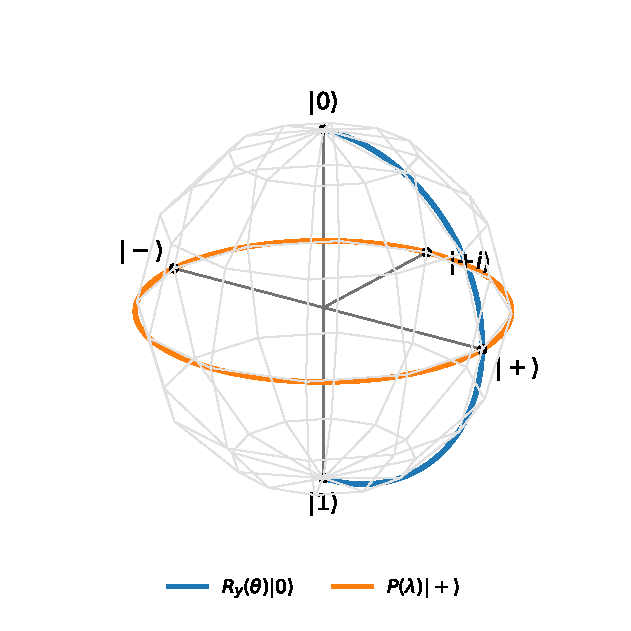
\includegraphics[width=0.48\textwidth]{rotation_paths}
\caption{Two rotation paths on the Bloch sphere. Blue: $R_y(\theta)\ket{0}$ for $\theta$ from 0 to $\pi$, a meridian from $\ket{0}$ to $\ket{1}$. Orange: $P(\lambda)\ket{+}$ for $\lambda$ from 0 to $2\pi$, the full equator.}
\label{fig:paths}
\end{figure}

Figure~\ref{fig:sweep} is Eq.~\eqref{eq:p1} tested two ways, in a seeded reproduction of the notebook's sweep: the exact probability from the state vector, and the fraction of 1s in 1000 shots at each of 25 angles. The worst of the 25 sampled points misses the curve by $0.049$, about three times the $\sqrt{p(1-p)/N} \le 0.016$ of Day~1. Two of the 25 points lie beyond three $\sigma$, which happens in roughly one sweep in fifteen; this seed drew a somewhat unlucky one, and that is itself the lesson: among many estimates, the extremes exceed $\sigma$.

\begin{figure}[h]
\centering
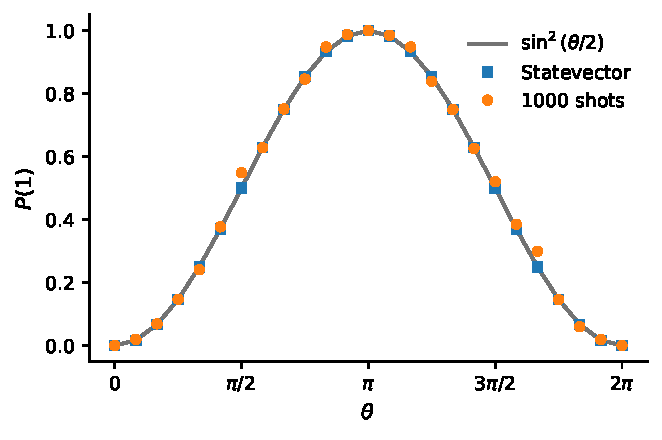
\includegraphics[width=0.58\textwidth]{ry_sweep}
\caption{$P(1)$ after $R_y(\theta)$ on $\ket{0}$: the curve $\sin^2(\theta/2)$, the exact value from \code{Statevector}, and the estimate from 1000 shots at each of 25 angles.}
\label{fig:sweep}
\end{figure}

\subsection{Phase gates}

A phase gate leaves $\ket{0}$ alone and multiplies $\ket{1}$ by $e^{i\lambda}$:
\begin{equation}
P(\lambda) = \begin{pmatrix}1&0\\0&e^{i\lambda}\end{pmatrix},\qquad
S = P(\pi/2) = \begin{pmatrix}1&0\\0&i\end{pmatrix},\qquad
T = P(\pi/4) = \begin{pmatrix}1&0\\0&e^{i\pi/4}\end{pmatrix},
\label{eq:phase}
\end{equation}
with $Z = P(\pi)$, so that $Z = S^2$ and $S = T^2$. Because the diagonal entries have magnitude one, $P(\lambda)$ changes neither $|\alpha|^2$ nor $|\beta|^2$: it changes only the relative phase, which Day~2 showed is the azimuth $\phi$ on the Bloch sphere. Applied to $\ket{+}$ it gives $(\ket{0} + e^{i\lambda}\ket{1})/\sqrt2$, whose Bloch vector is $(\cos\lambda, \sin\lambda, 0)$, a point on the equator at azimuth $\lambda$ (the orange path in Figure~\ref{fig:paths}). A phase gate is a rotation about $z$: $R_z(\theta)$ and $P(\theta)$ differ by exactly a global phase, $P(\theta) = e^{i\theta/2}R_z(\theta)$, which is why the notebook's checkpoints compare gates with \code{Operator.equiv} rather than with \code{np.allclose}.

\subsection{Every one-qubit gate}

Any $2\times2$ unitary is a rotation about some axis, and up to a global phase it can be written with three angles. Qiskit's general gate is
\begin{equation}
U(\theta,\phi,\lambda) = \begin{pmatrix}\cos\frac\theta2 & -e^{i\lambda}\sin\frac\theta2\\ e^{i\phi}\sin\frac\theta2 & e^{i(\phi+\lambda)}\cos\frac\theta2\end{pmatrix},
\label{eq:u}
\end{equation}
which is $R_z(\phi)R_y(\theta)R_z(\lambda)$ up to a phase; multiplying the three matrices of Eq.~\eqref{eq:rot} gives exactly $e^{-i(\phi+\lambda)/2}\,U(\theta,\phi,\lambda)$. This is the Euler-angle statement that any rotation of a sphere is a turn about $z$, then about $y$, then about $z$ again, and it is why a chip that can play $R_z$ and one fixed $x$-type rotation can produce every single-qubit gate. Its first column is the Bloch-sphere state of Day~2, so $U(\theta,\phi,\lambda)\ket{0}$ reaches any point on the sphere; $\lambda$ only matters for inputs other than $\ket{0}$. The Hadamard gate is not one of the named rotations, but it is $U(\pi/2, 0, \pi)$ exactly, and also $R_y(\pi/2)Z$ as matrices (in a circuit: $Z$ first, then $R_y(\pi/2)$). Geometrically $H$ is a half-turn about the axis halfway between $x$ and $z$, which is why it swaps the poles with $\ket{\pm}$.

\section{Composing gates}

A circuit is read left to right, but its matrix is the product of the gate matrices in the opposite order, because the first gate acts on the state first: a circuit with $A$ then $B$ has matrix $BA$. Day~2's $HZH = X$ is the matrix of the circuit \code{h; z; h}. Since gates need not commute, \code{x; h} and \code{h; x} are different circuits with matrices $HX$ and $XH$.

Every circuit can be undone. \code{inverse()} reverses the gate order and replaces each gate by its adjoint, so that for a circuit with matrix $U$ the inverse has matrix $U^\dagger$, and composing the two gives $U^\dagger U = I$. The reversal is forced by the identity $(BA)^\dagger = A^\dagger B^\dagger$: to undo $A$ then $B$, undo $B$ first. The notebook's Checkpoint builds \code{x; h}, computes \code{Operator(qc)}, and confirms it equals $HX$ and not $XH$; the two matrices are transposes of each other, and the difference is visible on $\ket{0}$, which $HX$ sends to $\ket{-}$ and $XH$ sends to $\ket{+}$.

\section{Measurement}

\subsection{Collapse}

The Born rule of Day~2 gives the probabilities. It also says what is left afterwards: if the outcome is $x$, the state after the measurement is $\ket{x}$. The superposition is gone, and on an ideal device a second measurement of the same qubit returns $x$ with certainty; on hardware, readout error and decay between the two readings make them disagree at the percent level. In Qiskit, \code{Statevector.measure()} returns both the outcome and the post-measurement state, and the notebook confirms that ten further measurements of that state all agree. In the projector language of Day~2, outcome $x$ occurs with probability $P(x) = \braket{\psi|P_x|\psi}$ and leaves the state $P_x\ket{\psi}/\sqrt{P(x)}$; a repeated measurement applies $P_x$ again, and $P_x^2 = P_x$ is the reason the answer cannot change. This is a \emph{projective measurement}, the only kind used in the bootcamp.

\subsection{Shots and the Sampler}

Repeating the circuit $N$ times gives counts that estimate the probabilities with the $\sqrt{Np(1-p)}$ spread of Day~1. Qiskit's \emph{primitives} are the interface that runs identically on a simulator and on hardware. The \emph{Sampler} takes circuits that end in measurements and returns counts:
\begin{lstlisting}
result = sampler.run([qc], shots=1000).result()
counts = result[0].data.meas.get_counts()   # from measure_all()
\end{lstlisting}
For $R_y(2\pi/3)\ket{0}$, where Eq.~\eqref{eq:p1} gives $P(1) = \sin^2(\pi/3) = 0.75$, the notebook's 1000 shots gave 778 ones, a fraction of $0.778$, about two standard deviations from the exact value and nothing unusual.

\subsection{Choosing the basis}

A measurement always asks ``0 or 1?'' along the $z$ axis. To ask the same question along another axis, first rotate that axis onto $z$, then measure. Table~\ref{tab:bases} lists the three standard choices. $H$ swaps $x$ and $z$, so an $H$ before the measurement reads the qubit in the $X$ basis $\{\ket{+},\ket{-}\}$; that is what Day~2 used to tell $\ket{+}$ from $\ket{-}$. For the $Y$ basis the rotation is $S^\dagger$ then $H$.

\begin{table}[h]
\centering
\small
\begin{tabular}{@{}llll@{}}
\toprule
basis & states & gates before measuring & outcome 0 means \\
\midrule
$Z$ & $\ket{0}, \ket{1}$ & none & $\ket{0}$ \\
$X$ & $\ket{+}, \ket{-}$ & \code{h} & $\ket{+}$ \\
$Y$ & $\ket{{+}i}, \ket{{-}i}$ & \code{sdg}, then \code{h} & $\ket{{+}i}$ \\
\bottomrule
\end{tabular}
\caption{Measuring in the three axis bases.}
\label{tab:bases}
\end{table}

The recipe behind the table is one rule. To measure in a basis $\{\ket{b_0}, \ket{b_1}\}$, apply the unitary $V$ that sends $\ket{b_0}\mapsto\ket{0}$ and $\ket{b_1}\mapsto\ket{1}$, then measure as usual; the outcome $k$ then means $\ket{b_k}$, with probability $|\braket{k|V|\psi}|^2 = |\braket{b_k|\psi}|^2$. For the $X$ basis $V = H$, since $H\ket{\pm} = \ket{0}, \ket{1}$; for the $Y$ basis $V = HS^\dagger$, since $S^\dagger$ first turns $\ket{{\pm}i}$ into $\ket{\pm}$. The same rule extends to any observable with a known eigenbasis, which is how Day~6 measures Pauli strings such as $XX$.

The state $\ket{{+}i} = S H\ket{0} = (\ket{0} + i\ket{1})/\sqrt2$ sits on the $y$ axis. Read in $Z$ or $X$ it is a fair coin; read in $Y$ it is certain (Figure~\ref{fig:bases}). The general rule is the Born rule with the basis states in place of $\ket{0}$ and $\ket{1}$: the probability of the outcome $\ket{b}$ is $|\braket{b|\psi}|^2$. For the notebook's prediction exercise, $\ket{\psi} = R_y(2\pi/3)\ket{0} = \cos\frac\pi3\ket{0} + \sin\frac\pi3\ket{1}$, this gives $P(0) = \cos^2\frac\pi3 = 0.250$ in the $Z$ basis and $P(+) = \tfrac12(\cos\frac\pi3 + \sin\frac\pi3)^2 = 0.933$ in the $X$ basis; 1000 shots each returned $0.244$ and $0.942$.

\begin{figure}[h]
\centering
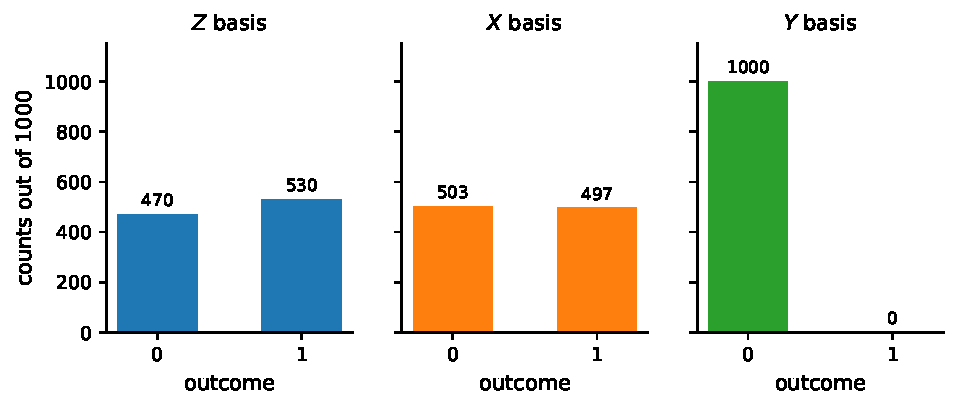
\includegraphics[width=0.85\textwidth]{three_bases}
\caption{$\ket{{+}i}$ read in the $Z$, $X$, and $Y$ bases, 1000 shots each: 470/530, 503/497, and 1000/0.}
\label{fig:bases}
\end{figure}

\section{Expectation values and the Estimator}

Assign the number $+1$ to outcome 0 and $-1$ to outcome 1 and average over shots. The average is the \emph{expectation value} of $Z$,
\begin{equation}
\braket{Z} = \braket{\psi|Z|\psi} = P(0) - P(1) = |\alpha|^2 - |\beta|^2 ,
\label{eq:expz}
\end{equation}
which is the $z$ coordinate on the Bloch sphere, as in Day~2. $\braket{X}$ and $\braket{Y}$ are the same average after the basis rotations of Table~\ref{tab:bases}. Estimated from $N$ shots, $\braket{Z}$ carries a statistical error of about $\sqrt{(1 - \braket{Z}^2)/N}$, which for $\ket{+}$ and $N = 1000$ is $0.03$. The formula is Day~1's binomial spread in new clothes: each shot contributes $+1$ or $-1$, a variable with mean $\braket{Z}$ and variance $1 - \braket{Z}^2$, and the average of $N$ such draws has variance $(1 - \braket{Z}^2)/N$. The error is largest for a 50/50 state and vanishes for an eigenstate, where every shot gives the same answer.

Any Hermitian matrix built from Paulis is an \emph{observable}, and the second primitive, the \emph{Estimator}, takes a circuit without measurements together with an observable and returns $\braket{\psi|O|\psi}$:
\begin{lstlisting}
job = estimator.run([(qc, SparsePauliOp("Z"))])
value = job.result()[0].data.evs
\end{lstlisting}
The two primitives divide the work between them (Table~\ref{tab:primitives}). Day~6 will hand a parameterized circuit to the Estimator and minimize the returned energy.

\begin{table}[h]
\centering
\small
\begin{tabular}{@{}lll@{}}
\toprule
& Sampler & Estimator \\
\midrule
input & circuits with measurements & circuits without measurements, plus observables \\
output & counts per outcome & one expectation value per observable \\
reads as & \code{data.meas.get\_counts()} & \code{data.evs} \\
used for & histograms, bitstring algorithms & energies, Bloch coordinates, cost functions \\
\bottomrule
\end{tabular}
\caption{The two Qiskit primitives.}
\label{tab:primitives}
\end{table}

\section{Two qubits}

\subsection{The tensor product}

Two qubits have four classical states, $00$, $01$, $10$, $11$, so their joint state is a vector of length four. When each qubit is in a state of its own, $\ket{a}$ and $\ket{b}$, the joint vector is the \emph{tensor product} $\ket{a}\otimes\ket{b}$, usually written $\ket{ab}$. Its entries are all the products of an entry of $\ket{a}$ with an entry of $\ket{b}$, in order:
\begin{equation}
\begin{pmatrix}a_0\\a_1\end{pmatrix}\otimes\begin{pmatrix}b_0\\b_1\end{pmatrix}
= \begin{pmatrix}a_0 b_0\\ a_0 b_1\\ a_1 b_0\\ a_1 b_1\end{pmatrix},
\qquad\text{so}\qquad
\ket{0}\otimes\ket{1} = \begin{pmatrix}0\\1\\0\\0\end{pmatrix} = \ket{01} .
\label{eq:kron}
\end{equation}
The entry at position $k$ is the amplitude of the bitstring that spells $k$ in binary. In numpy this is \code{np.kron(a, b)}. With $n$ qubits the vector has length $2^n$, and the amplitudes of the $2^n$ bitstrings are the state.

Gates combine the same way. A gate $A$ on one qubit and $B$ on the other act together as the $4\times4$ matrix $A\otimes B$, defined by $(A\otimes B)(\ket{a}\otimes\ket{b}) = A\ket{a}\otimes B\ket{b}$ and computed by \code{np.kron(A, B)}. A gate on one qubit alone is the tensor product with the identity on the other, and in Qiskit's ordering (next subsection) the left factor belongs to qubit~1, so \code{x(0)} is the matrix $I\otimes X$ and \code{x(1)} is $X\otimes I$. Pauli strings follow the same convention: the observable \code{"ZX"} is $Z\otimes X$ with $X$ on qubit~0. \code{Operator(qc)} returns the $4\times4$ matrix of a whole two-qubit circuit, and the notebook's Checkpoints compare it with these products.

\subsection{Qiskit's bit ordering}

Qiskit numbers qubits from the right. In the label \code{01}, qubit~1 is in $\ket{0}$ and qubit~0 is in $\ket{1}$, and the vector of Eq.~\eqref{eq:kron} is \code{np.kron(ket0, ket1)} with the \emph{left} factor belonging to qubit~1. A circuit that applies \code{x(0)} to $\ket{00}$ therefore produces the label \code{01}, not \code{10}. Counts dictionaries, \code{Statevector.from\_label}, and Pauli strings such as \code{"ZX"} all follow the same rule. Table~\ref{tab:order} spells it out for two qubits. Most textbooks write the control or the first qubit on the left; the physics is the same, and the two matrices are related by swapping the middle two rows and the middle two columns.

\begin{table}[h]
\centering
\small
\begin{tabular}{@{}lllll@{}}
\toprule
label & qubit 1 & qubit 0 & vector index & \code{np.kron} \\
\midrule
\code{00} & 0 & 0 & 0 & \code{kron(ket0, ket0)} \\
\code{01} & 0 & 1 & 1 & \code{kron(ket0, ket1)} \\
\code{10} & 1 & 0 & 2 & \code{kron(ket1, ket0)} \\
\code{11} & 1 & 1 & 3 & \code{kron(ket1, ket1)} \\
\bottomrule
\end{tabular}
\caption{Two-qubit labels, qubit values, and vector positions in Qiskit's convention.}
\label{tab:order}
\end{table}

\section{Product states and entangled states}

Not every length-4 vector is a tensor product. Arrange the four amplitudes as a $2\times2$ matrix $M$ with row index $q_1$ and column index $q_0$. For a product state Eq.~\eqref{eq:kron} gives $M_{ij} = a_i b_j$, which is an outer product and has rank one. Conversely a rank-one matrix factors as an outer product, so
\begin{equation}
\ket{\psi} \text{ is a product state} \iff \operatorname{rank} M = 1 .
\label{eq:rank}
\end{equation}
A state whose matrix has rank two cannot be written as $\ket{a}\otimes\ket{b}$ for any $\ket{a}$, $\ket{b}$. It is \emph{entangled}: neither qubit has a state of its own, only the pair does. The standard example is
\begin{equation}
\ket{\Phi^+} = \frac{1}{\sqrt2}\big(\ket{00} + \ket{11}\big), \qquad
M = \frac{1}{\sqrt2}\begin{pmatrix}1&0\\0&1\end{pmatrix}, \quad \operatorname{rank} M = 2 .
\label{eq:bell}
\end{equation}
The notebook's \code{is\_product} function is Eq.~\eqref{eq:rank} in one line: reshape \code{state.data} to $2\times2$ and ask \code{np.linalg.matrix\_rank} whether the rank is one. The rank test is a yes-or-no answer, but entanglement comes in degrees. The singular value decomposition of $M$ writes any two-qubit state as $\ket{\psi} = s_1\ket{a_1}\ket{b_1} + s_2\ket{a_2}\ket{b_2}$ with orthonormal $\ket{a_k}$, $\ket{b_k}$ and $s_1^2 + s_2^2 = 1$ (the \emph{Schmidt decomposition}); a product state has $s_2 = 0$, the Bell state has $s_1 = s_2 = 1/\sqrt2$, and $\cos\frac\pi8\ket{00} + \sin\frac\pi8\ket{11}$ lies between, with rank two but purity $\cos^4\frac\pi8 + \sin^4\frac\pi8 = 0.75$ for either qubit.

The same fact seen from one qubit: \code{partial\_trace} discards the other qubit and returns what is left, which is no longer a state vector but a \emph{density matrix} $\rho$. Its \emph{purity} $\operatorname{Tr}\rho^2$ is 1 for a pure state and $1/2$ for a 50/50 mixture of $\ket{0}$ and $\ket{1}$. For $\ket{+}\otimes\ket{1}$ the leftover qubit has purity 1; for $\ket{\Phi^+}$, which is maximally entangled, it has purity $1/2$; a partially entangled state lands in between. Alone, each qubit of a Bell pair is a coin with no phase at all; the information is entirely in the correlations.

\section{Two-qubit gates}

\subsection{CNOT}

Day~1 ended with the reversible table $(a,b)\mapsto(a, a\oplus b)$: keep the first bit, flip the second when the first is 1. As a gate it is \textsc{CNOT}, with a \emph{control} qubit and a \emph{target} qubit. In Qiskit \code{cx(0, 1)} has qubit~0 as control and qubit~1 as target. Reading off the four rows of Table~\ref{tab:order}, it fixes \code{00} and \code{10} (control 0) and exchanges \code{01} and \code{11} (control 1), so on the basis $\ket{00},\ket{01},\ket{10},\ket{11}$
\begin{equation}
\mathrm{CNOT}_{0\to1} = \begin{pmatrix}1&0&0&0\\0&0&0&1\\0&0&1&0\\0&1&0&0\end{pmatrix},
\quad
\mathrm{CZ} = \begin{pmatrix}1&0&0&0\\0&1&0&0\\0&0&1&0\\0&0&0&-1\end{pmatrix},
\quad
\mathrm{SWAP} = \begin{pmatrix}1&0&0&0\\0&0&1&0\\0&1&0&0\\0&0&0&1\end{pmatrix}.
\label{eq:gates}
\end{equation}
A textbook that puts the control on the left relabels $\ket{01} \leftrightarrow \ket{10}$, which swaps the middle two rows and the middle two columns of the same matrix (conjugation by SWAP). CNOT is a permutation matrix, so it is its own inverse: applied twice, nothing happened.

\subsection{CZ, SWAP, and controlled anything}

\textsc{CZ} applies $Z$ to the target when the control is 1. Since $Z$ only changes $\ket{1}$, the only effect is a minus sign on $\ket{11}$, and the matrix in Eq.~\eqref{eq:gates} is symmetric in the two qubits: control and target are interchangeable. \textsc{SWAP} exchanges the qubits, and the notebook's exercise builds it from three CNOTs in alternating directions,
\begin{equation}
\mathrm{SWAP} = \mathrm{CNOT}_{0\to1}\,\mathrm{CNOT}_{1\to0}\,\mathrm{CNOT}_{0\to1},
\end{equation}
which is the classical three-XOR swap. Any single-qubit gate $G$ has a controlled version, which with qubit~0 as control and qubit~1 as target is $I\otimes\ket{0}\bra{0} + G\otimes\ket{1}\bra{1}$ in the ordering of Table~\ref{tab:order} (left factor qubit~1), and Qiskit builds it with \code{gate.control()}.

\section{The Bell state}

Start from $\ket{00}$, apply $H$ to qubit~0, then CNOT with qubit~0 as control (Figure~\ref{fig:circuit}):
\begin{equation}
\ket{00} \xrightarrow{\;H\text{ on }q_0\;} \frac{1}{\sqrt2}\big(\ket{00} + \ket{01}\big)
\xrightarrow{\;\mathrm{CNOT}_{0\to1}\;} \frac{1}{\sqrt2}\big(\ket{00} + \ket{11}\big) = \ket{\Phi^+} .
\label{eq:bellprep}
\end{equation}
In the branch where $q_0 = 1$ the CNOT flips $q_1$ as well, so the two qubits end up agreeing in every branch. By Eq.~\eqref{eq:bell} the result has rank two and is entangled. Measured, it gives \code{00} or \code{11} and nothing else, each half the time; the notebook's 1000 shots gave 493 and 507.

\begin{figure}[h]
\centering
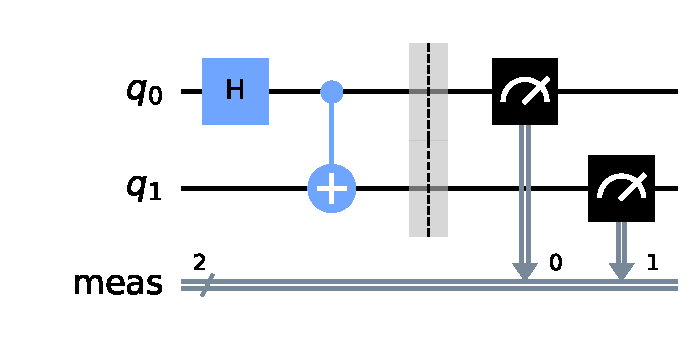
\includegraphics[width=0.36\textwidth]{bell_circuit}
\caption{The Bell circuit: $H$ on qubit 0, CNOT from qubit 0 to qubit 1, then measure both.}
\label{fig:circuit}
\end{figure}

There are four Bell states, reached from $\ket{\Phi^+}$ by single-qubit gates (Table~\ref{tab:bellstates}). $Z$ on either qubit flips the relative sign; $X$ on either qubit exchanges which pairs are correlated. All four are entangled, and they are orthogonal to each other, so together they form a basis of the two-qubit space: $\braket{\Phi^+|\Phi^-} = \tfrac12(1 - 1) = 0$, and $\Phi$ and $\Psi$ states share no basis vector at all. Because the four are reached from $\ket{\Phi^+}$ by gates on one qubit alone, a party holding one qubit of a shared Bell pair can steer the pair into any of the four without touching the other qubit, which is the mechanism behind superdense coding and teleportation.

\begin{table}[h]
\centering
\small
\begin{tabular}{@{}lll@{}}
\toprule
name & state & from $\ket{\Phi^+}$ \\
\midrule
$\ket{\Phi^+}$ & $(\ket{00} + \ket{11})/\sqrt2$ & \\
$\ket{\Phi^-}$ & $(\ket{00} - \ket{11})/\sqrt2$ & $Z$ on either qubit \\
$\ket{\Psi^+}$ & $(\ket{01} + \ket{10})/\sqrt2$ & $X$ on either qubit \\
$\ket{\Psi^-}$ & $(\ket{01} - \ket{10})/\sqrt2$ & $Z$ then $X$ \\
\bottomrule
\end{tabular}
\caption{The four Bell states.}
\label{tab:bellstates}
\end{table}

\section{Correlations in more than one basis}

Measuring both qubits of $\ket{\Phi^+}$ in the $Z$ basis always gives equal bits. On its own that is not remarkable: two coins glued heads-to-heads do the same. The difference appears when both qubits are read in the $X$ basis, with an $H$ on each before measuring (Table~\ref{tab:bases}). Substituting $\ket{0} = (\ket{+} + \ket{-})/\sqrt2$ and $\ket{1} = (\ket{+} - \ket{-})/\sqrt2$ into Eq.~\eqref{eq:bell} and collecting terms,
\begin{equation}
\ket{\Phi^+} = \frac{1}{\sqrt2}\big(\ket{{+}{+}} + \ket{{-}{-}}\big),
\label{eq:bellx}
\end{equation}
so the bits agree in the $X$ basis too. In expectation values, $ZZ$ is the observable that is $+1$ when the two $Z$ outcomes agree and $-1$ when they differ, and likewise $XX$. For the Bell state $\braket{ZZ} = \braket{XX} = 1$. A product state can score 1 on one of these but never both: $\ket{{+}{+}}$ has $\braket{XX} = 1$ but $\braket{ZZ} = 0$, since each qubit's $Z$ outcome is an independent fair coin. Figure~\ref{fig:corr} shows the four histograms and Table~\ref{tab:corr} the expectation values.

\begin{figure}[h]
\centering
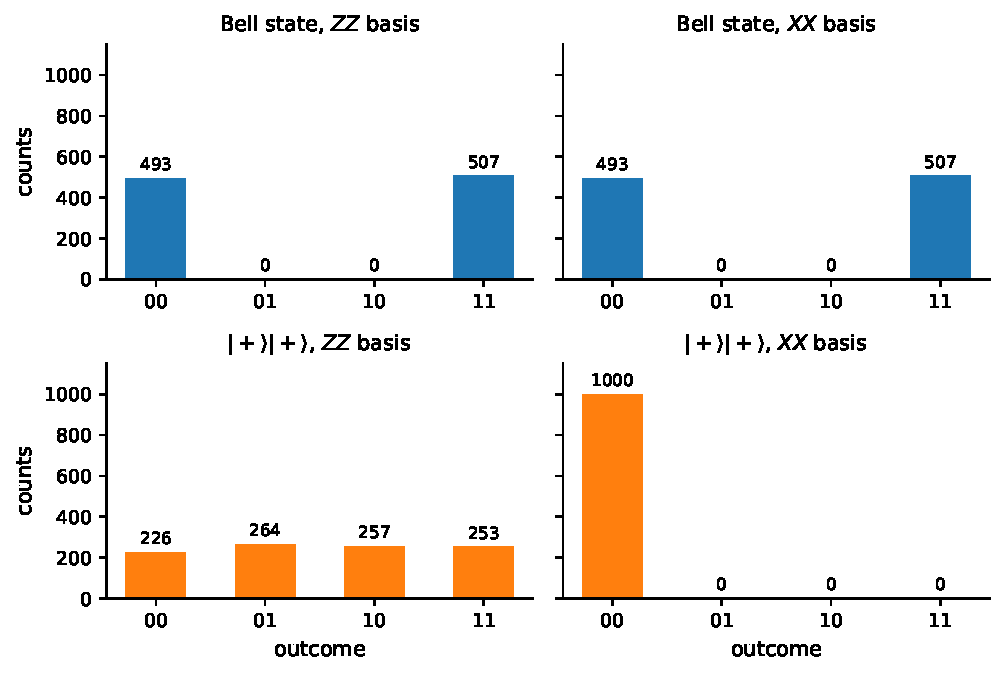
\includegraphics[width=0.8\textwidth]{correlations}
\caption{Both qubits measured in the $Z$ basis (left) and the $X$ basis (right), 1000 shots each. Top: the Bell state, correlated in both. Bottom: the product state $\ket{+}\ket{+}$, correlated in $X$ only.}
\label{fig:corr}
\end{figure}

\begin{table}[h]
\centering
\small
\begin{tabular}{@{}lllll@{}}
\toprule
state & $\braket{ZZ}$ & $\braket{XX}$ & $\braket{YY}$ & $\braket{ZX}$ \\
\midrule
$\ket{\Phi^+}$ & $1$ & $1$ & $-1$ & $0$ \\
$\ket{+}\ket{+}$ & $0$ & $1$ & $0$ & $0$ \\
\bottomrule
\end{tabular}
\caption{Two-qubit expectation values from the Estimator.}
\label{tab:corr}
\end{table}

The $Y$ basis completes the picture. In terms of $\ket{{\pm}i} = (\ket{0} \pm i\ket{1})/\sqrt2$ the same substitution gives $\ket{\Phi^+} = (\ket{{+}i,{-}i} + \ket{{-}i,{+}i})/\sqrt2$: the two bits now always \emph{differ}, $\braket{YY} = -1$, and the notebook's 1000 shots in the $Y$ basis gave 510 of \code{01} and 490 of \code{10}. Perfect correlations like these can still be reproduced by assigning each qubit definite values in advance: a pair of coins prepared with the same hidden list of answers for the $Z$, $X$, and $Y$ questions would agree and disagree in exactly the same pattern. Ruling that out takes measurements at intermediate angles. With $Z$ and $X$ on the first qubit and the rotated observables $(Z \pm X)/\sqrt2$ on the second, the combination
\begin{equation}
S = \braket{Z\otimes B_0} + \braket{Z\otimes B_1} + \braket{X\otimes B_0} - \braket{X\otimes B_1},\qquad B_{0,1} = \frac{Z \pm X}{\sqrt2},
\label{eq:chsh}
\end{equation}
can never exceed 2 if every outcome was fixed in advance, while the Bell state gives $S = 2\sqrt2 \approx 2.83$; each term is one \code{SparsePauliOp} handed to the Estimator. That is the CHSH inequality, the content of Bell's theorem, and the reading list has the details.

\section{GHZ states and the cost of $n$ qubits}

The Bell construction extends to any number of qubits. One $H$ followed by a chain of CNOTs, each copying the branch onto the next qubit, gives the \emph{GHZ state}
\begin{equation}
\ket{\mathrm{GHZ}_n} = \frac{1}{\sqrt2}\big(\ket{0\cdots0} + \ket{1\cdots1}\big),
\end{equation}
and the notebook's five-qubit version measured 498 of \code{00000} and 502 of \code{11111}. Every branch involves all $n$ qubits at once: measuring any single qubit collapses the whole register to one of the two bitstrings, and until then no qubit has a value of its own. Losing one qubit of a three-qubit GHZ state leaves the other two in a classical mixture of $\ket{00}$ and $\ket{11}$, with purity $1/2$: as with the Bell pair, the information is in the correlations, not in any one qubit.

A state vector of $n$ qubits holds $2^n$ complex numbers at 16 bytes each, so its memory is $2^n \times 16$ bytes and every added qubit doubles it (Figure~\ref{fig:memory}). The contrast with a classical register is the whole point: $n$ bits are described by $n$ numbers, $n$ qubits by $2^n$, because the state records an amplitude for every bitstring at once rather than one bitstring. At 30 qubits it is 16~GB, the whole memory of a laptop; at 40 it is 16~TB; at 45 it is half a petabyte, the largest full state vector that has actually been simulated; at 49 it is 9~PB, about all the memory of the largest supercomputer; at 56 it is an exabyte. This is why a quantum computer cannot be replaced by simulating one, and why Day~9 introduces simulators that do not store the full vector.

\begin{figure}[h]
\centering
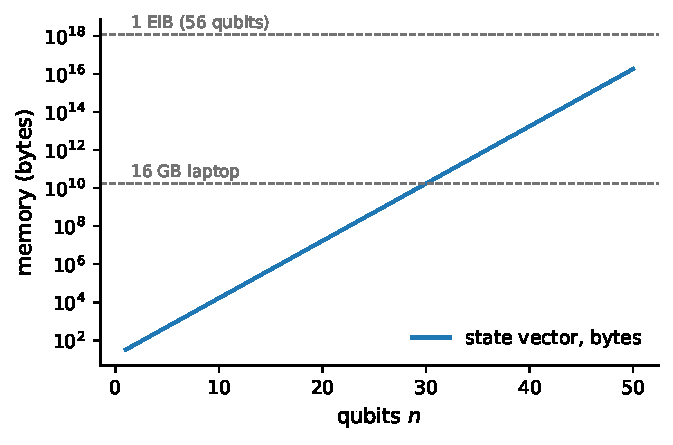
\includegraphics[width=0.58\textwidth]{memory_scaling}
\caption{Memory of a state vector against the number of qubits, with a laptop's 16 GB and one exabyte marked.}
\label{fig:memory}
\end{figure}

On hardware, the small bars at \code{01} and \code{10} that a Bell measurement returns, a few percent of the shots, are the first sign of the gate and readout errors that Day~5 measures one by one.

\section{Summary}

\begin{itemize}
\item The Paulis $X$, $Y$, $Z$, Eq.~\eqref{eq:pauli}, square to $I$, anticommute pairwise, and act as half-turns about their own Bloch axes.
\item Rotations $R_A(\theta) = \cos\frac\theta2 I - i\sin\frac\theta2 A$, Eqs.~\eqref{eq:rotexp} and~\eqref{eq:rot}, turn by $\theta$; $R_y(\theta)\ket{0}$ has $P(1) = \sin^2\frac\theta2$. Phase gates $P(\lambda)$, Eq.~\eqref{eq:phase}, rotate about $z$. Every one-qubit gate is $U(\theta,\phi,\lambda)$, Eq.~\eqref{eq:u}.
\item A circuit's matrix is the product of its gates in reverse order. Gates do not commute. \code{inverse()} gives $U^\dagger$.
\item Measurement collapses the state to the outcome. A rotation before measuring reads another basis: $H$ for $X$, $S^\dagger H$ for $Y$. The probability of outcome $\ket{b}$ is $|\braket{b|\psi}|^2$.
\item $\braket{Z} = P(0) - P(1)$, Eq.~\eqref{eq:expz}, is a Bloch coordinate. The Sampler returns counts; the Estimator returns expectation values of Pauli observables.
\item Two qubits are a length-4 vector; a product state is a tensor product, Eq.~\eqref{eq:kron}, computed with \code{np.kron}. Qiskit labels bitstrings with qubit 0 on the right (Table~\ref{tab:order}).
\item A two-qubit state is entangled when its $2\times2$ amplitude matrix has rank two, Eq.~\eqref{eq:rank}. Then neither qubit has a state of its own, and each looks like a mixture alone, 50/50 for the Bell state.
\item CNOT is Day~1's reversible XOR: it flips the target when the control is 1 and is its own inverse. CZ flips the sign of $\ket{11}$; SWAP exchanges qubits; any gate can be controlled, Eq.~\eqref{eq:gates}.
\item $H$ then CNOT makes the Bell state, Eq.~\eqref{eq:bellprep}; $Z$ and $X$ on one qubit reach the other three (Table~\ref{tab:bellstates}).
\item The Bell state's bits agree in the $Z$ and $X$ bases, Eq.~\eqref{eq:bellx}, and disagree in the $Y$ basis. No product state does all three (Table~\ref{tab:corr}).
\item GHZ generalizes Bell to $n$ qubits. A state vector costs $2^n \times 16$ bytes, which stops a laptop near 30 qubits and a supercomputer near 49.
\end{itemize}

\begin{thebibliography}{9}
\bibitem{watrous1} J.~Watrous, \emph{Basics of Quantum Information}, lesson 1, Single systems. IBM Quantum Learning. \url{https://quantum.cloud.ibm.com/learning/en/courses/basics-of-quantum-information/single-systems/introduction}
\bibitem{watrous2} J.~Watrous, \emph{Basics of Quantum Information}, lesson 2, Multiple systems. IBM Quantum Learning. \url{https://quantum.cloud.ibm.com/learning/en/courses/basics-of-quantum-information/multiple-systems/introduction}
\bibitem{nielsen} M.~A. Nielsen and I.~L. Chuang, \emph{Quantum Computation and Quantum Information}, 10th anniversary ed. (Cambridge University Press, 2010), sections 1.3, 2.2, 2.6 for Bell's theorem, and 4.2.
\bibitem{library} Qiskit API reference, circuit library, for the matrix of every gate. \url{https://quantum.cloud.ibm.com/docs/en/api/qiskit/circuit_library}
\bibitem{primitives} IBM Quantum documentation, \emph{Introduction to primitives}. \url{https://quantum.cloud.ibm.com/docs/en/guides/primitives}
\bibitem{ordering} IBM Quantum documentation, \emph{Bit-ordering in Qiskit}. \url{https://quantum.cloud.ibm.com/docs/en/guides/bit-ordering}
\bibitem{chsh} J.~F. Clauser, M.~A. Horne, A.~Shimony, and R.~A. Holt, ``Proposed experiment to test local hidden-variable theories,'' Phys. Rev. Lett. \textbf{23}, 880 (1969).
\end{thebibliography}

\end{document}
